\documentclass[12pt]{article}
% Machine Learning - COIY065H7\\Coursework Report
\usepackage[margin=1in,left=1.5in,includefoot]{geometry}
\usepackage{pythonhighlight}
% Header and Footer
\usepackage{fancyhdr}
\pagestyle{fancy}
%\fancyfoot{}
%\fancyfoot[R]{\thepage}

\usepackage{fullpage}
\usepackage{graphicx}
\usepackage{color}
\usepackage[usestackEOL]{stackengine}
\usepackage{url}
\usepackage{subfig}
\usepackage{multirow}
%\usepackage[table]{xcolor}
\usepackage{wrapfig}
\usepackage{blindtext}
\usepackage{amsmath,bm}
\usepackage{amssymb}
\usepackage{amsthm}
\usepackage{amsfonts}
%\usepackage[round]{natbib}
\usepackage{enumitem,xcolor}
\usepackage[multiple]{footmisc}

\usepackage{adjustbox}
\usepackage{kantlipsum}
\usepackage{tikz}
\usepackage[labelfont=bf]{caption}
\usepackage[utf8]{inputenc}
\usepackage{float}
% Default fixed font does not support bold face
\DeclareFixedFont{\ttb}{T1}{txtt}{bx}{n}{8} % for bold
\DeclareFixedFont{\ttm}{T1}{txtt}{m}{n}{8}  % for normal

% Custom colors
\usepackage{color}
\definecolor{deepblue}{rgb}{0,0,0.5}
\definecolor{deepred}{rgb}{0.6,0,0}
\definecolor{deepgreen}{rgb}{0,0.5,0}
\definecolor{coolblue}{HTML}{101094}

\usepackage{listings}
\lstset{%
   breaklines=true
}

\definecolor{codebg}{RGB}{238,238,238}

% Python style for highlighting
\newcommand\pythonstyle{\lstset{
    language=Python,
    basicstyle=\ttm,
    otherkeywords={},             % Add keywords here
    keywordstyle=\ttm\color{coolblue},
    emph={MyClass},          % Custom highlighting
    emphstyle=\ttm\color{deepred},    % Custom highlighting style
    stringstyle=\color{deepgreen},
    frame=tb,                         % Any extra options here
    framesep=10pt,
    framexleftmargin=10pt,
    backgroundcolor=\color{codebg},
    rulecolor=\color{codebg},
    aboveskip=15pt,
    belowskip=15pt,
    showstringspaces=false            % 
}}

% Python environment
%\lstnewenvironment{python}[1][] {
%    \pythonstyle
%    \lstset{#1}
%}{}

% Python for external files
\newcommand\pythonexternal[2][]{{
\pythonstyle
\lstinputlisting[#1]{#2}}}

% Python for inline
\newcommand\pythoninline[1]{{\pythonstyle\lstinline!#1!}}

\usepackage{biblatex}
\addbibresource{mlref.bib}

%\usepackage{amsmath}

\begin{document}

\begin{titlepage}
    \begin{center}
        \vspace*{.06\textheight}{\scshape\LARGE Birkbeck, University of London\par}\vspace{1.5cm} % University name
        \rule[0.5ex]{\linewidth}{2pt}\vspace*{-\baselineskip}\vspace*{3.2pt}
        \rule[0.5ex]{\linewidth}{1pt}\\[\baselineskip]
        %title of the report
        \huge{\bfseries Machine Learning - COIY065H7\\Coursework Report}\\[4mm]
        \rule[0.5ex]{\linewidth}{1pt}\vspace*{-\baselineskip}\vspace{3.2pt}
        \rule[0.5ex]{\linewidth}{2pt}\\
        [2.5cm]
    
        \textsc{\Large Baran Buluttekin\\13153116\\bbulut02@dcs.bbk.ac.uk}\\
        [1.5cm]
        \large \textit{ I have read and understood the sections of plagiarism in the College Policy on assessment offences and confirm that the work is my own, with the work of others clearly acknowledged. I give my permission to submit my report to the plagiarism testing database that the College is using and test it using plagiarism detection software, search engines or meta-searching software.}


    \end{center}
    \cleardoublepage
\end{titlepage}   


\pagenumbering{roman}
\section*{Abstract}
\addcontentsline{toc}{section}{Abstract}

This report is the summary for my findings in classification of the yeast dataset \cite{data}. In the introduction general information is given about the dataset and challenges associated with this problem is laid out. Section 2 gives an background information about techniques and algorithms that will be used to solve the problem. Methodology section gives more detailed breakdown of the steps for solution. Experiments and results section will introduce metrics and summary statistics obtained from the experiments. Conclusion section will highlight general findings and offer a next steps for the improvement. 

There is also appendix section at the end that includes python code used to carry out the experimentations. Even though it will produce the results of the experiments it will take a while to run due to the high number of experimentations and parameter tuning used. Therefore please consider using jupyter notebook provided with the submission to reproduction.

\clearpage

\tableofcontents
\thispagestyle{empty}
\clearpage

\pagenumbering{arabic}
\setcounter{page}{1}


\section{Introduction} \label{sec:introduction}
This report is part of the coursework for \textit{Machine Learning} (COIY065H7) module. From the coursework instructs Yeast data \cite{data} has chosen as the dataset.

\subsection{Dataset} \label{subsec:data}

Yeast dataset is part of the UCI machine learning repository where variety of machine learning related datasets curated. This dataset includes properties of yeast proteins to predict localization site of the protein. Number of data points in the dataset is 1484 and have 9 features in which only 8 of them are predictive feature. First feature is only index indicating database of that data acquired and have no predictive purpose. Final column of the data set provides label for protein class that we are aiming to predict. This dataset have no missing values. Given the labelled nature of the data this classification problem can be solved using \textit{supervised learning}.

\subsubsection{Problem Statement} \label{subsec:problem}

There are some additional properties of this data makes classification task challenging. Firstly this is a multi class classification problem, because our dataset have 10 distinct labels. Labels extracted from dataset are, 'MIT', 'NUC', 'CYT', 'ME1', 'EXC', 'ME2', 'ME3', 'VAC', 'POX' and 'ERL'. Secondary challenge is that this dataset have class imbalance. Number of instances varies form 463 observation of 'CYT' to 5 instances of 'ERL'.

\section{Algorithms and Techniques} \label{sec:algo}

There are number of techniques and algorithms introduced to address the challenges mentioned in the subsection \ref{subsec:problem}. I will list some of this techniques below and explain more detailed in the fallowing sections.

\begin{itemize}
    \item \textbf{Over-sampling data: }This method oversample the minority class in the data to create balanced classes.
    \item \textbf{Under-sampling data: }Opposite of the item above this method under sample the majority class to balance the data.
    \item \textbf{Balanced sampling for ensemble: }Sampling data in a balanced way while building ensemble models.
    \item \textbf{Choosing performance matrix sensitive to imbalance: }Using evaluation metric such as f1 score instead of accuracy will better capture mis-classification errors.
\end{itemize}

Most of the techniques discussed above are implemented as a code package in imbalance-learn \cite{imbalancelearn}. In the case of over-sampling, only random sampling method available for multi class datasets. Choice of algorithm for under-sampling is substantially more than over-sampling. But due to the very large gap in the number of instances in the different classes, under-sampling can effect performance of the classification model significantly. For example if we were to under-sample until we reached to balance dataset because of the only 5 instance in the class 'ERL' we would get a dataset of 50 instances (10 class times 5 observation each). Regardless I will be using alternative under-sampling algorithm design to experiment their performance. 

\subsection{Under-sampling methods} \label{subsec:undersample}

In addition to random under-sampling method special algorithms to under-sample selectively will be used in experiments. One such algorithm is \textit{Condensed nearest neighbour} (CNN) \cite{condense}, utilizes one nearest neighbor rule to decide for each instance to be removed from the dataset or not. Algorithm steps from the article are \cite{condense}:

\begin{quote}
    "Get all minority samples in a set \textit{C}.

    Add a sample from the targeted class (class to be under-sampled) in C and all other samples of this class in a set \textit{S}.


    Go through the set S, sample by sample, and classify each sample using a 1 nearest neighbor rule.

    If the sample is misclassified, add it to C, otherwise do nothing.

    Reiterate on \textit{S} until there is no samples to be added."
\end{quote}

\textit{Neighbor cleaning rule} (NCL) \cite{neighborcleaning} is another algorithm that derived from CNN where more emphasis give to the data cleaning.

\subsection{Sampling for ensemble} \label{subsec:ensemble}

Ensemble models uses subset of the data with replacement while training different classifier but this sapling usually does not take class imbalance into account. Classifiers in the imbalance-learn library build in a way that sampling is done while maintaining the class balance. Below is the short description of these classifiers.

\textit{Balanced random forest} \cite{rforestbalanced} classifier is design such a way that each bootstrap sample to train tree in the forest is supplied with balanced class subset.
This algorithm uses classic random forest \cite{randomforest} implementation and only differs in the sampling methodology.


\textit{RUSBoost} \cite{rusboost} also randomly sample data in balanced way before the boosting implemented.

\textit{Easy Ensemble} \cite{adaboostbalance} is an AdaBoost \cite{adaboost} implementation trained on balanced bootstrap samples.

\section{Methodology} \label{sec:method}
As an initial step, I have loaded the dataset in a data frame using Pandas \cite{pandas} package which then allow for exploratory examination of the data. For that reason I have created a pairplot to observe if there is any linear separation is possible. Please fallow the steps of the code snippet below to reproduce the visualization. All variable in the data is paired to each other except the "pox" and "erl" which behaves more like categorical data then continuous data.

Base line machine algorithms like random forest, AdaBoost, Support vector classifier and others are part of Scikit-learn \cite{scikit-learn} package. All visualization created are achieved using Matplotlib \cite{matplotlib} and Seaborn \cite{seaborn} software packages. For reproducibility random number state is chosen and in variable named as RANDOM\_STATE. All non-deterministic algorithm uses this random generator seed.

\begin{python}
import pandas as pd
import seaborn as sns
import matplotlib.pyplot as plt

url = "https://archive.ics.uci.edu/ml/machine-learning-databases/yeast/yeast.data"
columns = ["mcg", "gvh", "alm", "mit", "erl", "pox", "vac", "nuc", "class"]
df = pd.read_csv(url, header=None, sep=r"\s+", names=columns, usecols=list(range(1,10)))

feature_list = [x for x in df.columns if x not in ['pox', 'erl']]
# Plotting
sns.pairplot(df[feature_list], hue='class')
\end{python}

\begin{figure}[H] \label{fig:pairplot}
    \centering
    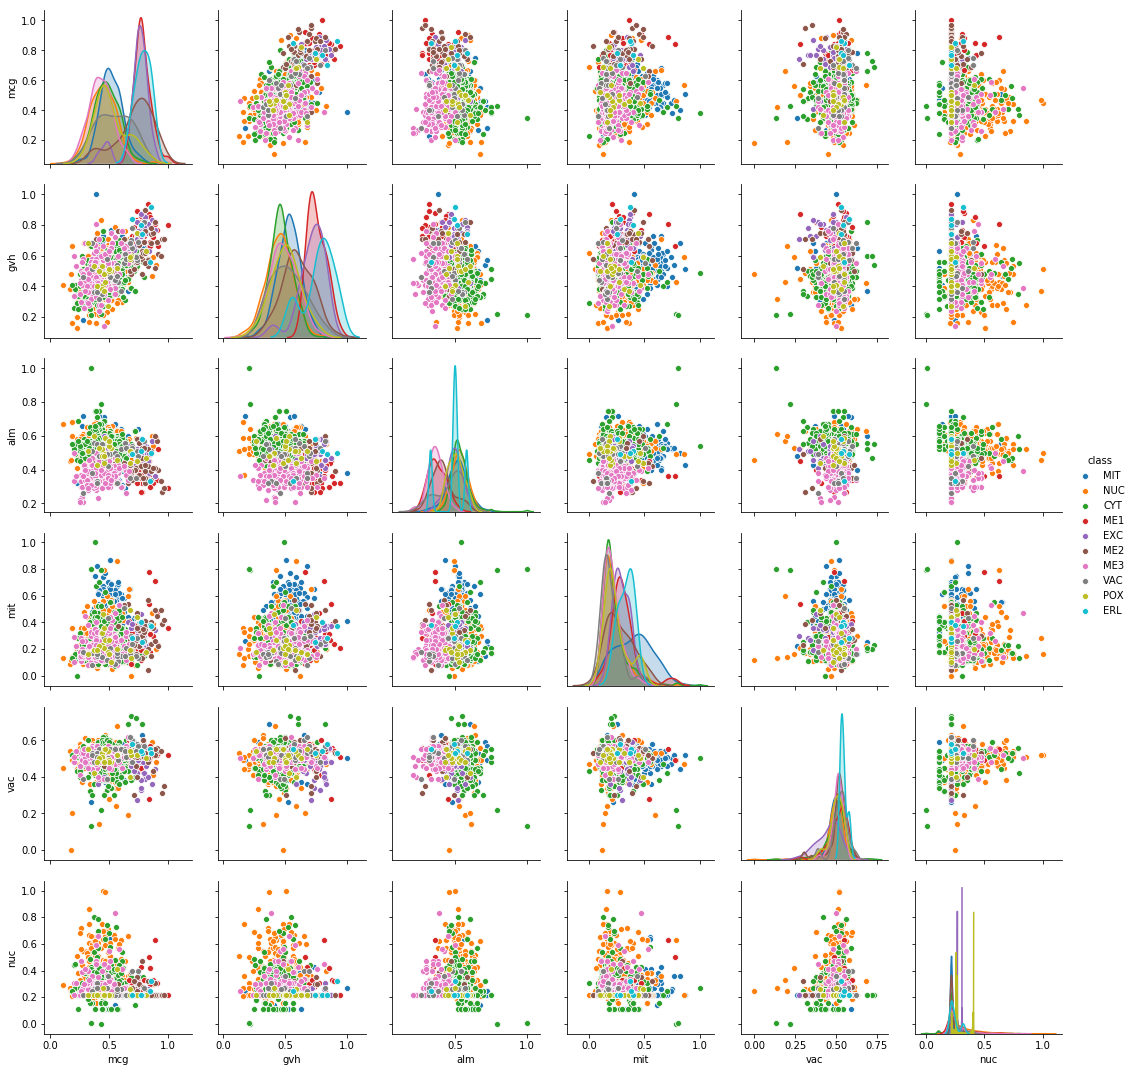
\includegraphics[width=\textwidth]{img/pairplot.png}
    \caption{Pairplot of the data.}
\end{figure}

\subsection{Data preprocessing} \label{subsec:preprocess}
Data preprocessing is relatively simple for this dataset. There are no missing values and all data points are numeric which only leaves us to encode class variable to be able to feed into machine learning model. Judging from pairplot above classes have different range in some variable and can benefit min max scaling of the data. 

In later stages some regularization algorithms will be applied to data to observe its effects in the generalization.

This preparation can be streamlined with fallowing code.

\begin{python}
    def process_data(df):
        encoder = LabelEncoder()
        y = encoder.fit_transform(df['class'])
        X = df[df.columns[:-1]].values
        return X, y

    def process_scaled_data(df):
        l_encoder = LabelEncoder()
        scaler = MinMaxScaler()
        y = l_encoder.fit_transform(df['class'])
        X = df[df.columns[:-1]].values
        X = scaler.fit_transform(X)
        return X, y
\end{python}

\subsection{Over-sampling and training model} \label{subsec:oversample}
Defined over-sampling method will be applied and compare the result with the same classifier trained on the data to observe if over-sampling help the classification task. Similarly utility function is created for the ease of transformation.

\begin{python}
    def make_over_sample(X, y, random_state=0):
        ros = RandomOverSampler(random_state=random_state)
        return ros.fit_resample(X, y)
\end{python}

\subsection{Under-sample and train model} \label{subsec:compareundersample}

I previously discuss that we have different algorithm for under-sampling and details for these algorithms given in the subsection \ref{subsec:undersample}. These algorithms implemented in imbalance-learn package as \textit{CondensedNearestNeighbour}, \textit{NeighbourhoodCleaningRule} and \textit{RandomUnderSampler}. Similarly these will be compared to base models trained on the data to evaluate if under-sampling helps the classification. Also implemented with utility function.

\begin{python}
    def make_under_sample(X, y, method=NeighbourhoodCleaningRule, random_state=0):
        clf = method(random_state=random_state)
        return clf.fit_resample(X, y)
\end{python}

\subsection{Comparison of models} \label{subsec:comparison}

All of the experimentations will be carried out by firstly splitting data to training and testing data. For the splitting \textit{StratifiedKFold} algorithm is chosen because of the minority class in the dataset. If the random splitting algorithm is used minority class can either not represented in test data or training data. StratifiedKFold will ensure each class is represented in the training and test dataset. All machine learning algorithm and sampling techniques will be applied to training data after the split so the effect of each process can be examined on unseen data when it tested with test data. This rule also applies to any scaling on the data. Applying scaling separately to test and training data especially important because applying scaling before splitting will cause information leakage and will cause to misleading results in testing.

Main choice of evaluation metric for this classification is f1 score because of its nature of combining precision and recall. F1 score calculates as harmonic mean of precision and recall, calculated with formula:

\begin{equation*}
    H = \frac{n}{\frac{1}{x_{1}} + \frac{1}{x_{2}} + \cdots + \frac{1}{x_{n}}} = \frac{n}{\sum_{i=1}^n{\frac{1}{x_{i}}}}
\end{equation*}

\begin{equation*}
    F_{1} = \frac{2}{\frac{1}{precision} + \frac{1}{recall}} = 2 \times \frac{precision \times recall}{precision + recall}
\end{equation*}
Harmonic mean differ from arithmetic mean in a way that it will give more weight to low value, hence f1 score will increase only if both precision and recall increases.

For each experimentation I will use Random forest, AdaBoost, logistic regression, and svm classifier to observe and compare performance of each method.

Random forest classifier is an ensemble of decision trees that uses the bagging method. Data points and the features are sampled from data to create diverse set of trees. AdaBoost is also an ensemble model that uses bootstrap bagging but mainly differ by assigning a weigh and then emphasising an error in prediction with these weight to build an bagging model. Both of these algorithms will be tuned using number of trees which is implemented in the scikit-learn as "n\_estimators".

Logistic regression classifier is similar to logistic regression which fits a mathematical model to underlie data and optimizing parameters $\theta$ together with a bias term $\theta_{0}$.

\begin{gather*}
    \hat{y} = \theta_{0} + \theta_{1}x_{1} + \theta_{2}x_{2} + \cdots + \theta_{n}x_{n} \\
     \hat{y} = \theta^T \cdot x
\end{gather*}

Then this fitter equation passed to \textit{logit} function to make a prediction between 2 class (0 and 1)

\begin{equation*}
    \sigma(z) = \frac{1}{1 + e^{-z}} = \frac{1}{1 + e^{-\theta^T \cdot x}}
\end{equation*}

Despite being originally design as binary classification algorithm it can be applied to multi class classification as well. In scikit-learn this can be achieved by using multi\_class=”multinomial” option in the instance.


In general first over-sampling and under-sampling method will be compared to classification models build on original data. Then another comparison will be drawn on balanced ensemble models versus general ensemble models which later all will be compared. This process will be repeated on the scaled data to observe scaling effect. All models will be trained with hyper-parameter tuning using cross validation.

\section{Experiments and Results} \label{sec:experiment}
\subsection{Ensemble models performance} \label{subse:ensemblemodelperformance}
Selected ensemble models first trained with different hyper-parameters and best performing parameter selected to fit the data using number of estimators in all of the classifiers. Table below summarize the maximum f1 score for each classifier in training and test data. Furthermore all ensemble models trained in [100, 200, 300, 400, 500] numbers of trees and their f1 score observed as well as plotted to below graph. Performance of the algorithm on test set drawn using dotted line and test set score drawn in solid line using same color.

\begin{center}
    \begin{tabular}{||c c c||} 
    \hline
    Classifier & F1 score (training) & F1 score (test)\\ [0.5ex] 
    \hline\hline
    RandomForestClassifier & \textbf{1.0} & \textbf{0.6686} \\ 
    \hline
    AdaBoostClassifier & 0.3670 & 0.3892 \\
    \hline
    EasyEnsembleClassifier & 0.5001 & 0.5917 \\
    \hline
    BalancedRandomForestClassifier & 0.4890 & 0.5148 \\
    \hline
    BalancedBaggingClassifier & 0.5633 & 0.6035\\ [1ex] 
    \hline
   \end{tabular}
\end{center}

If we observe the f1 score of all the classifiers in the all n\_estimators we can see after the random forest best performing imbalanced ensemble model was BalancedBaggingClassifier.

\begin{figure}[H] \label{fig:ensemblepf}
    \centering
    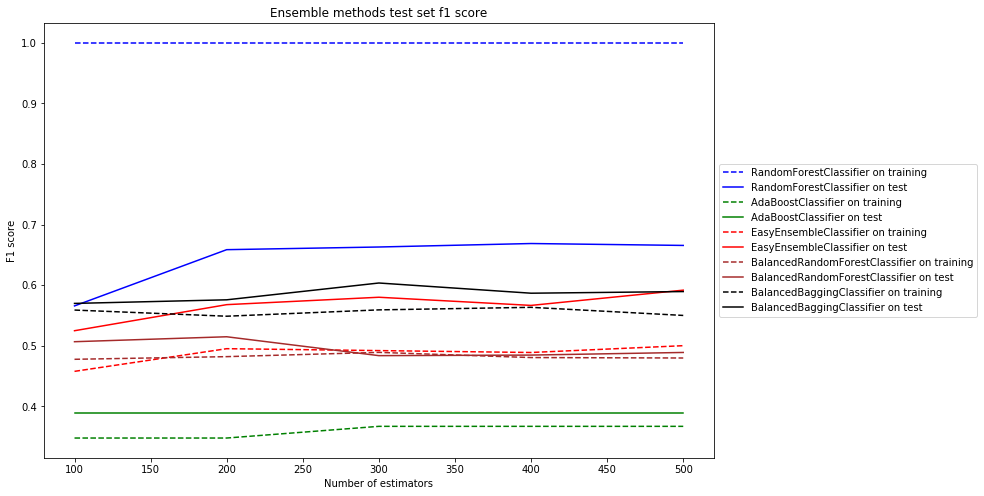
\includegraphics[width=\textwidth]{img/ensembletestf1.png}
    \caption{F1 score of ensemble models.}
\end{figure}

We can investigate RandomForestClassifier predictions further by visualizing its confusion matrix. Which show each number of correctly classified prediction in each class.

\begin{figure}[H] \label{fig:rfconfusion}
    \centering
    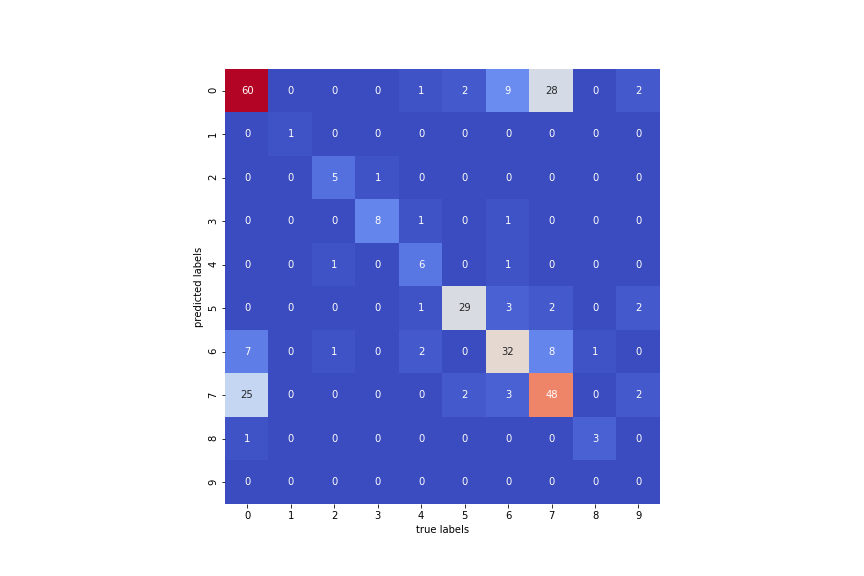
\includegraphics[width=\textwidth]{img/rfheatmap.png}
    \caption{Confusion matrix of RandomForestClassifier.}
\end{figure}

We can see that "CYT" (0) class is often mis-classified as "NUC" (7) and vice versa. Rest of the classes predicted well.

\subsection{Over-sampling v baseline classifiers}
As a first step over sampled dataset made available with the random over-sampling defined in subsection \ref{subsec:oversample}, number of class instances in the over-sampled data. Presented below.

\begin{center}
    \begin{tabular}{||c c c||} 
    \hline
    Class & Over-sampled instances & Training dataset instances\\ [0.5ex] 
    \hline\hline
    0 & 370 & 370\\ 
    \hline
    1 & 370 & 4\\
    \hline
    2 & 370 & 28\\
    \hline
    3 & 370 & 35\\
    \hline
    4 & 370 & 40\\
    \hline
    5 & 370 & 130\\
    \hline
    6 & 370 & 195\\
    \hline
    7 & 370 & 343\\
    \hline
    8 & 370 & 16\\
    \hline
    9 & 370 & 24\\ [1ex] 
    \hline
   \end{tabular}
\end{center}

Similar to previous subsection I trained ensemble models using number of tree parameter "n\_estimators" from 100 to 1000 incrementing 100 in each training. Same algorithm first train in the training data and them trained on over-sampled dataset. F1 scores are tested in training dataset and test data. Below is the change of the performance metric over the number of trees in the algorithm. Algorithm trained on the over-sample data denoted with "\_o" at the end of algorithm such as "RandomForestClassifier\_o".

\begin{figure}[H] \label{fig:overscomp}
    \centering
    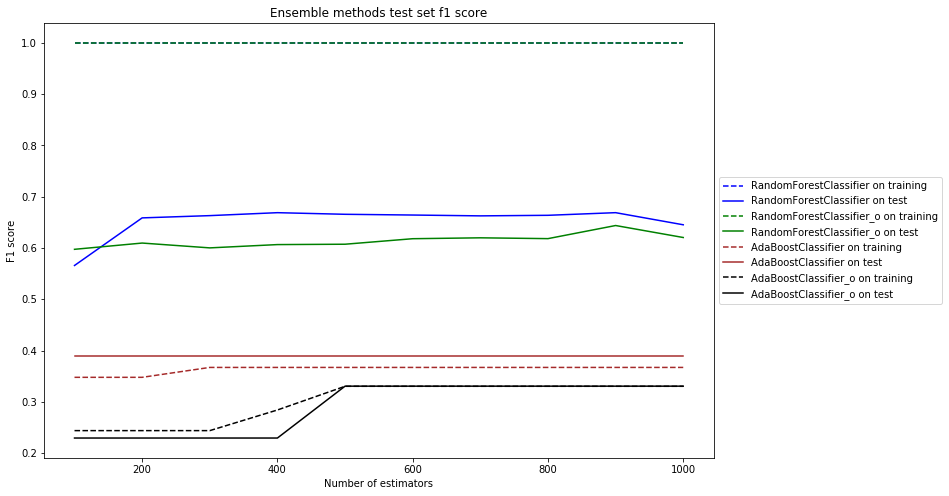
\includegraphics[width=\textwidth]{img/ensembleoversample.png}
    \caption{Over-sampled v base classifiers.}
\end{figure}

Both random forest and the AdaBoost performed slightly better when they trained base dataset. 

Logistic regression and support vector classifier (SVC) also trined in the both dataset to check if over-sampled data have different effect on algorithms that are not ensemble algorithms. Both of these algorithms performed slightly better in the over-sampled data than base dataset. Summary score for all the algorithms presented below.

\begin{center}
    \begin{tabular}{||c c c c c||} 
    \hline
    \multicolumn{5}{||c||}{F1 Scores} \\
    \hline
    Algorithm & \multicolumn{2}{c}{Base Dataset} & \multicolumn{2}{c||}{Over-sampled} \\
    Name & Training & Test & Training & Test \\ [0.5ex] 
    \hline\hline
    RandomForest & 1.0 & 0.6686 & 1.0 & 0.6436\\ 
    \hline
    AdaBoost & 0.3670 & 0.3892 & 0.3302 & 0.3305\\ 
    \hline
    SVC & 0.5923 & 0.5981 & 0.5980 & 0.6069\\ 
    \hline
    LogisticRegression & 0.5847 & 0.5542 & 0.5105 & 0.5568\\ [1ex] 
    \hline
   \end{tabular}
\end{center}

\subsection{Under-sampling v baseline classifiers} \label{subsec:undervbase}

Experimentation from previous section repeated for all the algorithms used in the previous section for the under sampling.
Algorithms for under-sampling discussed in subsection \ref{subsec:compareundersample} and the dataset instances produced by using these presented below.

\begin{center}
    \begin{tabular}{||c c c c c||} 
    \hline
    Class  & Dataset & RUS & CNN & NCL\\ [0.5ex] 
    \hline\hline
    0 & 370 & 4 & 2 & 243\\ 
    \hline
    1 & 4 & 4 & 4 & 4\\
    \hline
    2 & 28 & 4 & 1 & 17\\
    \hline
    3 & 35 & 4 & 1 & 25\\
    \hline
    4 & 40 & 4 & 2 & 10\\
    \hline
    5 & 130 & 4 & 2 & 86\\
    \hline
    6 & 195 & 4 & 2 & 95\\
    \hline
    7 & 343 & 4 & 4 & 162\\
    \hline
    8 & 16 & 4 & 2 & 7\\
    \hline
    9 & 24 & 4 & 2 & 0\\ [1ex] 
    \hline
   \end{tabular}
\end{center}

For the case of under-sampling algorithms trined on original training set out performed under-sampled peers overwhelmingly for random under-sampling (RUS) and CondensedNearestNeighbour (CNN). NeighbourhoodCleaningRule (NCL) on the other hand performed slightly worse than baseline. These results were expected for the under-sampling case because of the reason that very few data points left in the dataset for most of the under-sampling technique. Full performance comparison provided in the table below.

\begin{center}
    \begin{tabular}{||c c c c c c c c c||} 
    \hline
    \multicolumn{9}{||c||}{F1 Scores} \\
    \hline
    Algorithm & \multicolumn{2}{c}{Base Dataset} & \multicolumn{2}{c}{RUS} & \multicolumn{2}{c}{CNN} & \multicolumn{2}{c||}{NCL}\\
    Name & Training & Test & Training & Test & Training & Test & Training & Test\\ [0.5ex] 
    \hline\hline
    RandomForest & 1.0 & 0.6686 & 0.3946 & 0.4287 & 0.2708 & 0.2509 & 0.6366 & 0.6362\\ 
    \hline
    AdaBoost & 0.3670 & 0.3892 & 0.1330 & 0.1807 & 0.05153 & 0.0446 & 0.2903 & 0.3160\\ 
    \hline
    SVC & 0.5923 & 0.5981 & 0.3356 & 0.3830 & 0.1450 & 0.1447 & 0.5619 & 0.5887\\ 
    \hline
    LogisticRegression & 0.5847 & 0.5542 & 0.3276 & 0.3978 & 0.3291 & 0.3187 & 0.6023 & 0.5937\\ [1ex] 
    \hline
   \end{tabular}
\end{center}

\subsection{Using regularization} \label{subse:scalingdata}

As a final comparison dataset is scaled with min max regularizer from scikit-learn \cite{scikit-learn} package. Ensemble classifiers trained on base dataset and scaled dataset to compare the effect of scaling in the data. Performance of the scaled data was considerably lower than the classifier trained on original data. One reason for this performance reduction can be relative power of the data has a fundamental importance as we can see in the confusion matrix that common mis-classification between classes increases when scaling applied to the dataset.

\begin{figure}[H] \label{fig:scalecomp}
    \centering
    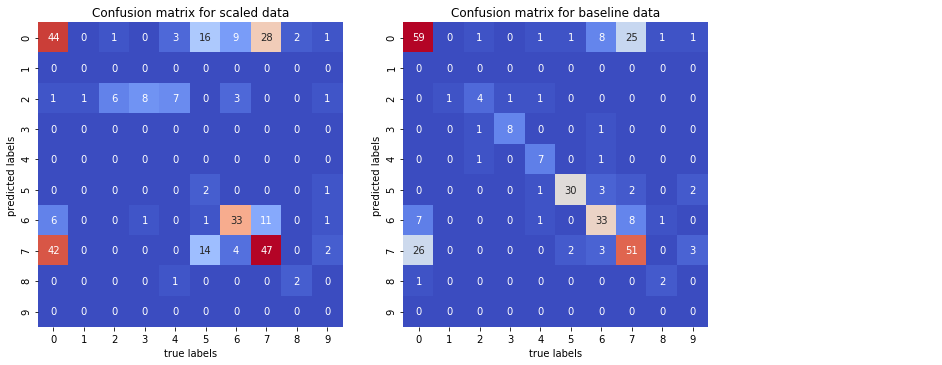
\includegraphics[width=\textwidth]{img/confusioncompare.png}
    \caption{Comparison of same Random forest model in scaled and baseline data.}
\end{figure}

\section{Conclusion} \label{sec:conclution}

In conclusion, common imbalance techniques had very limited impact on this classification problem. Under-sampling algorithms was not successful mostly because of large number of data loss when the technique applied. Over-sampling and balanced sample bootstrapped ensemble algorithms had similar performance to predictions those without. Albeit slightly less successfully. In general combination of very steep difference in imbalance of the classes and having moderately small data kept this classification problem still a challenging task.

Further improvements can be achieve by training different models or trying additional techniques such as stacking to gain more accuracy.

\printbibliography
\addcontentsline{toc}{section}{References}

\section*{Appendix}
\addcontentsline{toc}{section}{Appendix}
\lstinputlisting[language=Python]{ml_coursework.py}
\end{document}
